\documentclass[a4paper, 11pt]{article}

%%% Zeichenkodierung, Rechtschreibung und Umlaute
\usepackage[utf8]{inputenc}
\usepackage[ngerman]{babel}
\usepackage[T1]{fontenc}

%%% Mathematische Symbole, Gleichungen
\usepackage[fleqn]{amsmath}
\usepackage{amsfonts}
\usepackage{amssymb}
\usepackage{amsthm}
\usepackage{mathtools}
\usepackage{bm}
%\usepackage{colonequals} % Zusätzliche Relationssymbole

%%% Tabellen
\usepackage{tabularx}
\usepackage{array}
\usepackage{multicol}

%%% Seitenformat und -ränder
%%% -Alternative 1-
\usepackage{geometry}
\geometry{a4paper, top=25mm, bottom=20mm, left=20mm, right=20mm}
%%% -Alternative 2-
%\usepackage[headheight=110pt]{geometry}
%\geometry{a4paper,left=30mm,right=30mm, top=35mm, bottom=30mm}

%%% Seitenstile (Kopf- und Fußzeile)
\usepackage{fancyhdr}
\pagestyle{fancy}

%%% Sonstiges
\usepackage{caption} % Untertitel von Grafiken/Tabellen manipulieren
\usepackage{enumerate} % Aufzählungszeichen ändern
\usepackage{graphicx} % Standarderweiterung für Bilddateien
\usepackage{hyperref} % Hyperlinks
\usepackage{lastpage} % Berechnung der Seitenzahl
%\usepackage{polynom} % Polynomdivision
\usepackage{setspace} % Zeilenabstand
%\usepackage{textgreek} % griechische Symbole
\usepackage{tikz} % Umfassendes Tool, um Grafiken zu erstellen
\usepackage{verbatim} % Schreibmaschinen-Stil (für Code-Ausschnitte)
\usepackage{float}

%%% Eingaben (z.B. für das Deckblatt)
\newcommand{\module}{Embedded System Design -- Protokoll}
\newcommand{\semester}{Sommersemester 2018}
\newcommand{\finishingdate}{29.06.2018}
\newcommand{\titletext}{Video  Audio Streaming} %TODO: Nummer anpassen

%%%-- Für das Deckblatt --
\title{
	~\\[4cm]
	\textbf{
		\module\\[0.25cm]
		\normalsize \semester \\[1.5cm]
		\Huge\titletext\\
	}
}

\author{
  \vspace{3.5cm}\\
  \begin{tabular}{l}
    \textbf{Gruppe 15:}\\\hline
    Omid Rahimian Mashhadi \\
    Torsten Michael Schenk\\
  \end{tabular}
}

\date{
	\vfill
	Abgabedatum: \finishingdate\\
	\vspace{5mm}
	Seitenanzahl: \pageref{LastPage}
}

%%% -- Kopf- und Fußzeile --
%%% Kopfzeile linker Bereich
\lhead[\leftmark]{\textbf{\module}}
%%% Kopfzeile mittlerer Bereich
\chead[\rightmark]{\rightmark{\titletext}}
%%% Kopfzeile linker Bereich
\rhead{\textbf{zum \finishingdate}}
%%% Fußzeile
\cfoot{\thepage  \ / \pageref{LastPage}}

%%% Serifenfreie Fonts benutzen
%\renewcommand{\familydefault}{\sfdefault}

%%% Font
\usepackage{charter}

%%% Tiefe der Einrückung nach Absätzen
\setlength{\parindent}{0pt}

%%% Evtl. Änderungen des Typs einer Aufzählungsebene (z.B. zur Anpassung an das Aufgabenblatt)
%\renewcommand{\labelenumi}{\alph{enumi})}
%\renewcommand{\labelenumii}{(\roman{enumii})}
%\renewcommand{\labelenumiii}{\arabic{enumiii}.}
%\renewcommand{\labelenumii}{\textbf{-}}

\begin{document}

%%% Deckblatt
\maketitle
\thispagestyle{empty} % Keine Seitenzahl hier
\newpage

%%% Seitenzahl zurücksetzen
\clearpage
\setcounter{page}{1}

%%% Zeilenabstand
%\singlespacing
\onehalfspacing
%\doublespacing

%%%-- Eigentlicher Inhalt --
\section*{Aufgabe 1: }

Eine Funktion $f : \mathbb{R}^3 \to \mathbb{R}$ sollte folgende Kriterien erfüllen, um eine implizite Fläche zu beschreiben.\\

Um Innen von Außen unterscheiden zu können: \\
$f(P_1) > 0$ und $f(P_2) < 0$ \hspace{5pt} $\Rightarrow$ \hspace{5pt} Auf jedem Weg zwischen $P_1$ und $P_2$ gibt es eine Nullstelle.\\

Um wirklich eine Fläche und kein Volumen von Nullstellen zu erhalten:\\
Es gibt kein $P \in \mathbb{R}^3$ und $r \in \mathbb{R}$ mit $r > 0$, sodass für alle $x \in \mathbb{R}^3$ mit $\lVert P - x \rVert < r$ gilt $f(x) = 0$.


\section{h264}

Beschreibung des Projektes...


\begin{minipage}{\textwidth}
    \begin{center}
        Caption for image
        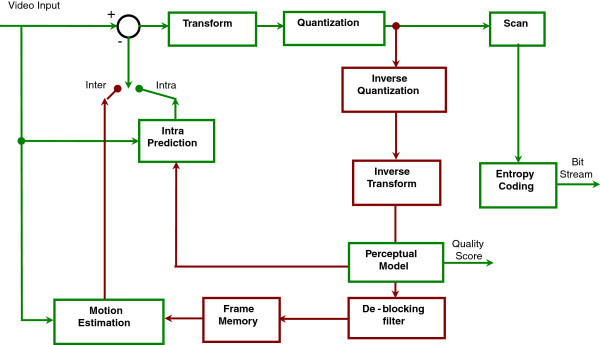
\includegraphics[scale=4.0]{img/h264.jpg} 
    \end{center}
\end{minipage}



\section{gstreamer}

Wenn Fehler beim Compilieren eines gstream Testprogramms auftreten, z.B.
\begin{verbatim}
Package gstreamer-1.0 was not found in the pkg-config search path.
Perhaps you should add the directory containing `gstreamer-1.0.pc'
to the PKG_CONFIG_PATH environment variable
No package 'gstreamer-1.0' found
playback-tutorial-6.c:1:10: fatal error: gst/gst.h: No such file or directory
\end{verbatim}

gstreamer-1.0 ist der folgenden lib enthalten:\\
sudo apt install libgstreamer1.0-dev\\

\textbf{Beispiel Programme gstreamer kompilieren}
gcc playback-tutorial-6.c -o playback-tutorial-6 `pkg-config --cflags --libs gstreamer-1.0`

\section{Strato Web Server}

\textbf{Login via ssh}\\
ssh -X root@85.214.211.169\\
ssh -X root@85.214.211.169 -L 5901:localhost:5901\\
pwd: xxxxxxxxxx (pwd vom Provider)

\textbf{Remote Desktop}\\
tightvncserver: server\\
xtightvncviewer: viewer\\
sudo apt install tightvncserver xtightvncviewer\\
\# set xtightvnciewer pwd\\

\textbf{Full Login}\\
ssh -X root@85.214.211.169 -L 5901:localhost:5901\\
ssh Passwort eingeben\\
\# Start vncserver\\
vncserver :1\\
echo \grqq{}\$DISPLAY\grqq{}\\
\# in server ssh console\\
xtightvncviewer 127.0.0.1:1\\
vnc Passwort eingeben\\
\# X Fenster sollte sich öffnen








\newpage
\section{Rapsi Touchscreen Display}

\# Zeige Namen aller angeschlossenen Displays\\
xrandr -q\\

\# 180 Grad drehen\\
xrandr --output HDMI-1 --rotate inverted\\

\# Touchscreen muss auch rotiert werden\\
\# bitte einfügen in /boot/config.txt:\\
\# rote touchscreen (display rotated via xrandr startup script)\\
lcd\_rotate=2\\



\section{noch eins}

\section*{Definitionen Fachbegriffe:}

Test

\end{document}
